\documentclass[UTF8]{ctexart}
\CTEXsetup[format={\Large\bfseries}]{section}
\usepackage[a4paper,left=3cm,right=3cm,top=2cm]{geometry}
\usepackage{amsmath}
\usepackage{enumitem}
\usepackage{float}
\usepackage{threeparttable}
\usepackage{caption}
\usepackage{multirow}
\usepackage{graphicx}
\usepackage{listings}
\usepackage{color}

\definecolor{dkgreen}{rgb}{0,0.6,0}
\definecolor{gray}{rgb}{0.5,0.5,0.5}
\definecolor{mauve}{rgb}{0.58,0,0.82}
\lstset{
  frame=tb,
  language=C++,
  aboveskip=3mm,
  belowskip=3mm,
  showstringspaces=false,
  columns=flexible,
  basicstyle={\small\ttfamily},
  numbers=left,%设置行号位置none不显示行号
  %numberstyle=\tiny\courier, %设置行号大小
  numberstyle=\tiny\color{gray},
  keywordstyle=\color{blue},
  commentstyle=\color{dkgreen},
  stringstyle=\color{mauve},
  breaklines=true,
  breakatwhitespace=true,
  escapeinside=`,%逃逸字符(1左面的键),用于显示中文例如在代码中`中文...`
  tabsize=4,
  extendedchars=false %解决代码跨页时,章节标题,页眉等汉字不显示的问题
}

\setlength\lineskiplimit{5.25bp}
\setlength\lineskip{5.25bp}

\title{计算方法编程作业2\ 实验报告}
\author{崔士强 PB22151743}
\date{\today}

\bibliographystyle{plain}

\begin{document}

\maketitle
\section{原理}
\subsection{初始化}
根据实验文档给出的原理,我们可以为解方程组做如下准备:
\begin{enumerate}
  \item 初始化系数矩阵$\mathbf{A}$. 
  
  首先创建一个$n-1$行全$0$方阵,再遍历每个位置,对应设置数值.
  \item 初始化向量$\mathbf{b}$. 
  
  由给出的差分方程可以知道,$\mathbf{b}$除了最后一个分量外全为$ah^2$,最后一个分量为$ah^2-(\epsilon + h)$,由此可以初始化$\mathbf{b}$.
\end{enumerate}

\subsection{列主元Gauss消元法}
在程序中定义一个类\lstinline|GaussianElimination|用于列主元Gauss消元法的计算,其中定义了\lstinline|void Solve()|成员函数, 
首先通过另一个成员函数\lstinline|int SelectMax(int i)|选出最大行,与当前行进行交换,然后消去接下来所有行的首个非零元素,最后回代.

\subsection{Gauss-Seidel迭代}
构造函数接收$\mathbf{A}$, $\mathbf{b}$, 以及算法的容差(用于结束判断). 初始向量设为全$0$向量,然后通过一个\lstinline|while|循环
进行迭代,如果两次结果各个分量差方和的平方根小于容差则退出循环.

\section{实验结果}
\subsection{数值结果}
大部分结果误差较小,在$0.1\%$以下,另外观察到以下规律:
\begin{enumerate}
  \item 对于两种方法,均发现越靠近$0$,百分比误差越大,原因是更小的数值对误差更敏感.
  \item 总体上来说,随着$\epsilon$的减小,误差随之减小,然而观察到在最接近$0$的几个点处误差非常大,超过了$3\%$,推测原因与上一条所述类似.
\begin{figure}[h]
    \centering
    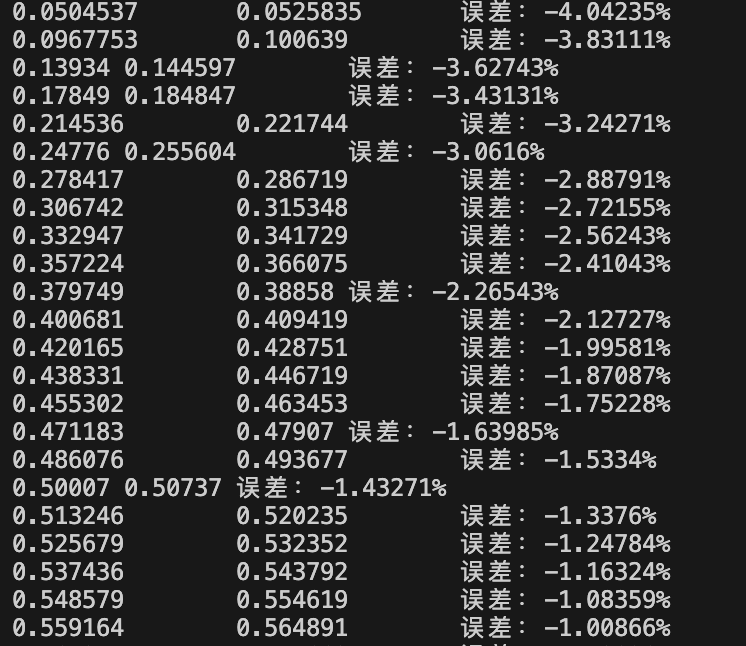
\includegraphics[scale=0.5]{pic1.png}
    \caption{靠近0处较大的误差}
\end{figure}
  \item 两种方法的误差没有明显区别.
\end{enumerate}

\subsection{运行时间}
对于几组不同$\epsilon$的输入,两种算法的运行时间($\mu s$)如下表所示.

\begin{table}[H]
  \centering
  \begin{tabular}{ccccc}
    \hline
    $\epsilon$ & 1 & 0.1 & 0.01 & 0.0001 \\
    \hline \hline
    Gauss消元 & 4992 & 1476 & 1542 & 1475 \\
    Gauss-Seidel迭代 & 386444 & 147130 & 5224 & 4324 \\
    \hline
  \end{tabular}
\end{table}

总体上来说,Gauss消元法的运行速度更快,Gauss-Seidel迭代在处理$\epsilon$值更小的矩阵时时间明显缩短,推测原因是此时矩阵谱半径更大.

\bibliography{math}

\end{document}
\iffalse
\begin{figure}[h]
    \centering
    \includegraphics[scale=0.5]{name.png}
    \caption{name}
\end{figure}
\fi
